\section{LoRa module}
In order to test the LoRa SX1278 module, one wrote a small program to test send and receive functions from LoRa module, with the usage shown in figure \ref{fig:loratest}.

\begin{figure}[H]
	\centering	
	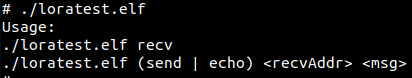
\includegraphics[width=0.6\textwidth]{13tests/lora/loratest}
	\caption{Test LoRa module.}
	\label{fig:loratest}
\end{figure}

Using two LoRa modules, one was connected to a Raspberry Pi in\linebreak
\verb|tomas-abreu|'s computer with local address defined as \verb|0xbb|, the other was connected to another Raspberry Pi in \verb|fernandes|'s computer with local address \verb|0xcc|.

One tested the read and send functions of the module, firstly by waiting for a message, as shown in figure \ref{fig:loratest_recv}.

\begin{figure}[H]
	\centering	
	\includegraphics[width=0.6\textwidth]{13tests/lora/BB_recv_wait}
	\caption{Test LoRa module: waiting for receive.}
	\label{fig:loratest_recv}
\end{figure}

In figure \ref{fig:loratest_send} (a) the device \verb|0xcc| sends the message \verb|"Hello from 0xCC"| to the device \verb|0xbb|, presenting all the attributes, from the source address, \verb|'from'| field, to the destination address, \verb|'to'| field, including also message attributes, as the \verb|msgID|, \verb|msgLength| and the \verb|msg| itself.

In figure \ref{fig:loratest_send} (b) is shown the receiver side, receiving the message correctly, with error 0, and presenting all the attributes from the received message, matching all that were sent by the sender.

\begin{figure}[H]%
	\centering
	\subfloat[\centering Sender side ]{{\includegraphics[width=6.25cm]{13tests/lora/CC_send}}}%
	\qquad
	\subfloat[\centering Receiver side ]{{\includegraphics[width=6.25cm]{13tests/lora/BB_recv}}}%
	\caption{Test LoRa module: send message from 0xcc to 0xbb.}%
	\label{fig:loratest_send}%
\end{figure}
	
As previously seen, the SPI interface works by sending two bytes in a row, depending on what operation it is: read or write. In figure \ref{fig:loratest_sck_nss} is seen the clock signal (SCK, in red) and the slave select signal (NSS, in yellow).

\begin{figure}[H]
	\centering	
	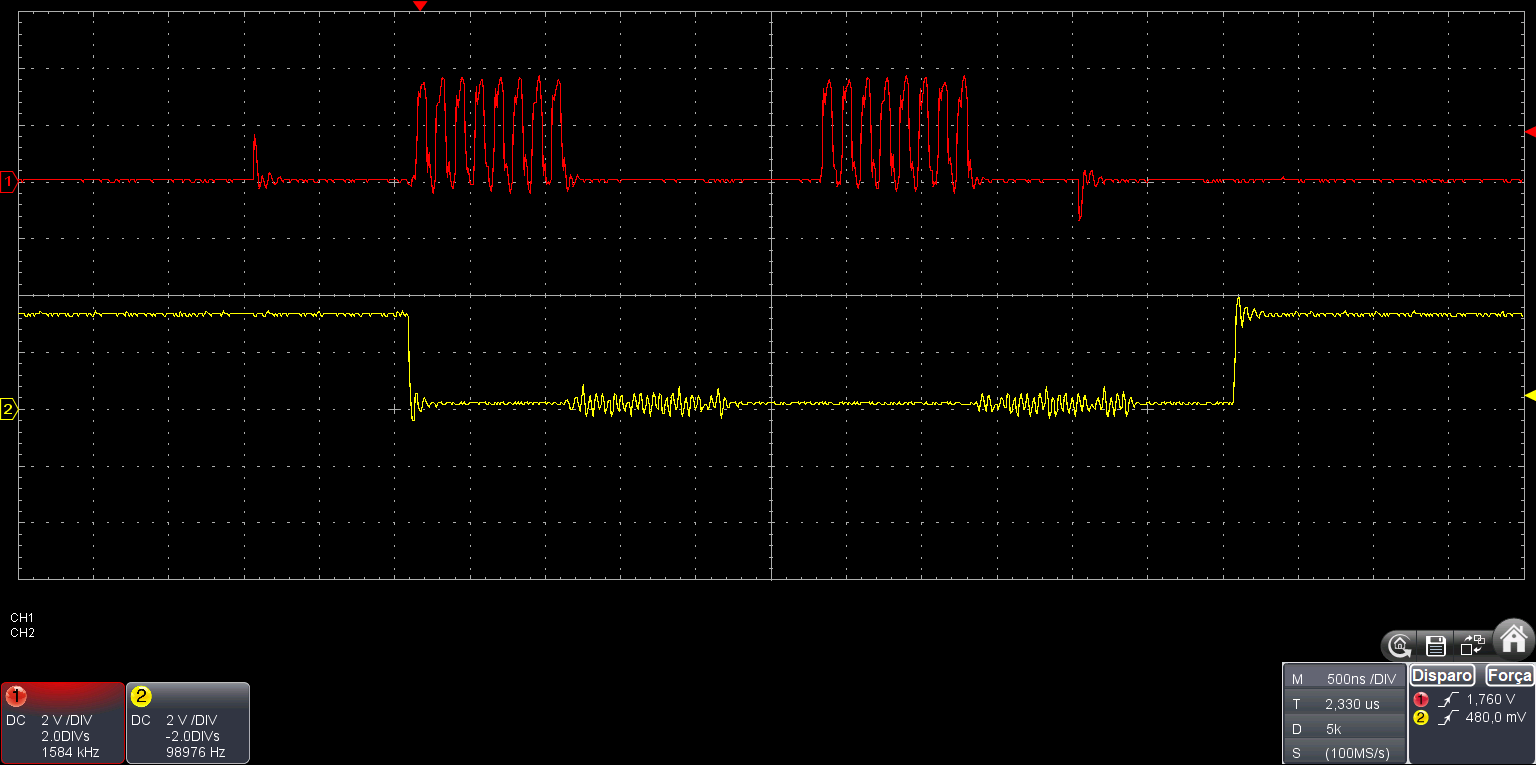
\includegraphics[width=1\textwidth]{13tests/lora/SCK_CS}
	\caption{Test LoRa module: SCK (in red) and NSS (in yellow) signals.}
	\label{fig:loratest_sck_nss}
\end{figure}

When the NSS goes to low, a transfer is started, with the master generating SCK. For each byte are generated 8 pulses of clock, 1 pulse per bit sent. Due to overhead and delays introduced by the software, there is a gap between the two bytes sent, where the NSS signal is still low but the SCK is not being generated. When NSS goes high, the transfer is over.

%**********************************************************
\section{TSL2581}
After the I2C configuration, one can see that the TSL2581 was detected in the bus by the Raspberry Pi, by running the command \verb|i2cdetect -y 1|. The execution of this command detects all the devices connected to the I2C bus and, as seen in the figure \ref{fig:i2cDetect}, it detects the TSL2581 device with its default address, 0x39, as seen before \ref{section:lumSensor}. One can also see what type of operations are allowed to this device, by running the command \verb|i2cdetect -F 1|.

\begin{figure}[H]
	\centering	
	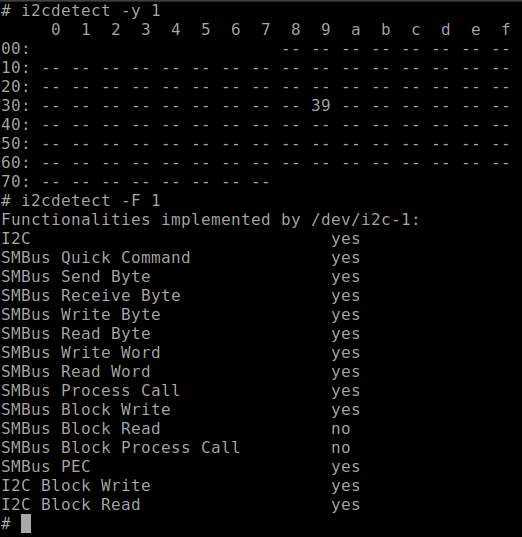
\includegraphics[width=.6\textwidth]{13tests/ldr/i2c_detect}
	\caption{Test TSL2581 module: device detection in I2C bus.}
	\label{fig:i2cDetect}
\end{figure}

After the device was detected in the I2C bus, one wrote a small program to test the values read by the sensor module. The figure \ref{fig:testtsl} shows the execution of the test program, \verb|testtsl.elf|, that prints the values read from the sensor every second.

\begin{figure}[H]
	\centering	
	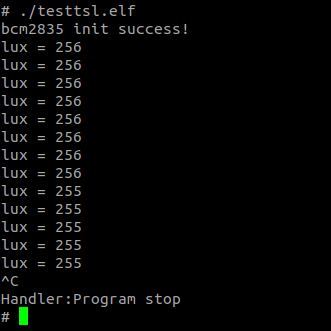
\includegraphics[width=.5\textwidth]{13tests/ldr/testtsl}
	\caption{Test TSL2581 module: Test program for TSL2581.}
	\label{fig:testtsl}
\end{figure}

As previously seen, the I2C communication protocol uses a clock line and a data line. The communications start by the master sending the slave address to the bus, and if the correspondent slave responds, then the master can send other commands to the slave. In figure \ref{fig:i2c_SCL_SDA} is presented the clock line (SCL), in red, and the data line (SDA), in yellow, and shows that in the first eight bits of clock, the master sends the slave address \verb|0x39|. In the next eight bits of clock, the master sends a command to read the low byte of the \textit{Channel\_0}, being the command sent by the master equal to \verb|0xD4|.

\begin{figure}[H]
	\centering	
	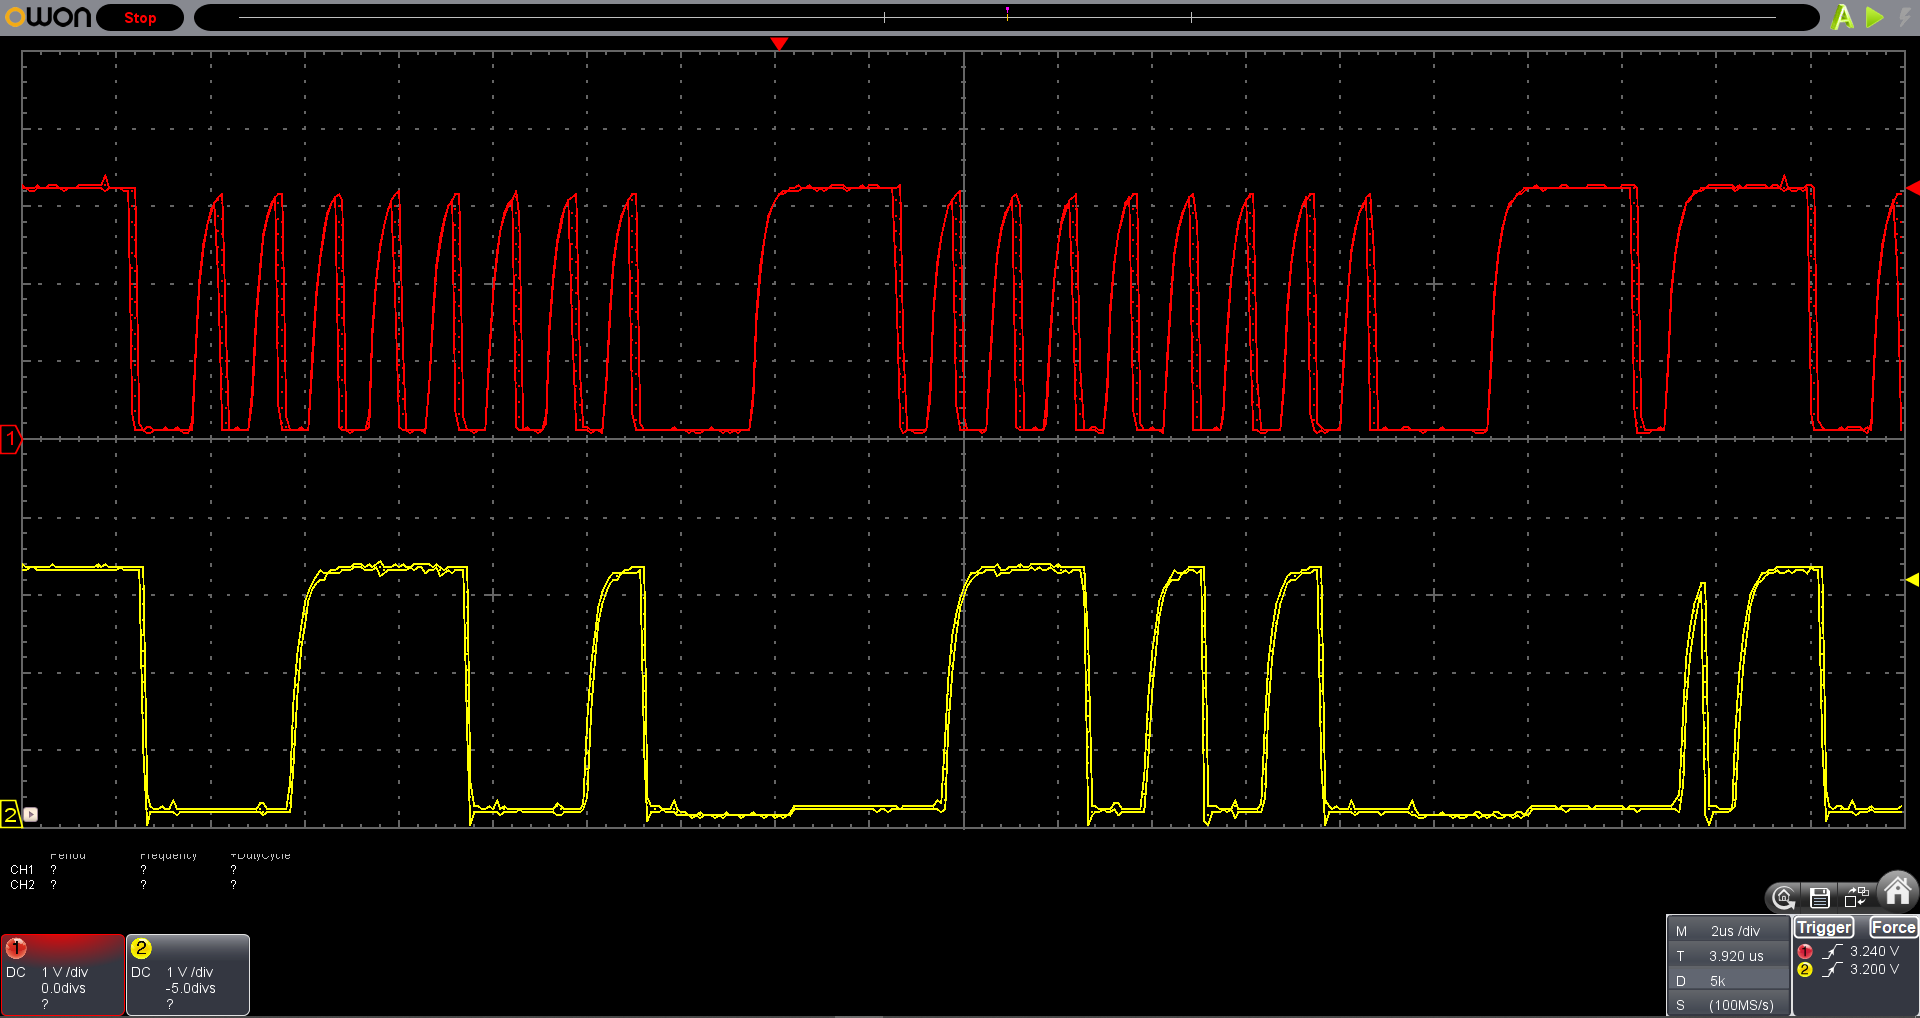
\includegraphics[width=1\textwidth]{13tests/ldr/scl_sda_i2c}
	\caption{Test TSL2581 module: Transmission of two bytes: SCL (in red) and SCK (in yellow) signals.}
	\label{fig:i2c_SCL_SDA}
\end{figure}

The figure \ref{fig:tsl} shows the montage of the TSL2581 with the Raspberry Pi, with the interrupt pin not being used.

\begin{figure}[H]
	\centering	
	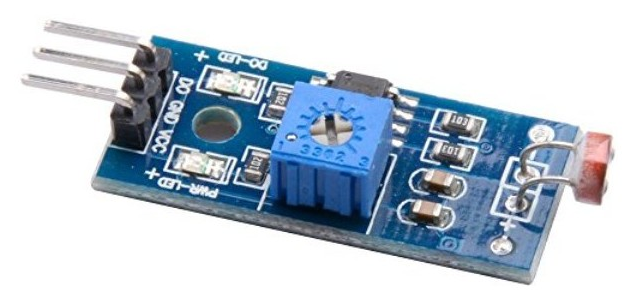
\includegraphics[width=.9\textwidth]{13tests/ldr/ldr}
	\caption{Test TSL2581 module: Montage.}
	\label{fig:tsl}
\end{figure}

%**********************************************************
\section{PWM control}
In order to test PWM control, one wrote a small program to test the generation of a PWM signal at 50 Hz with a variable duty cycle, with the usage shown in figure \ref{fig:loratest}. The duty cycle received is a value from 0 to 1.

\begin{figure}[H]
	\centering	
	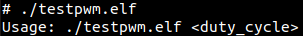
\includegraphics[width=.5\textwidth]{13tests/pwm/testpwm}
	\caption{Test PWM control.}
	\label{fig:testpwm}
\end{figure}

In figure \ref{fig:pwm_50} one defined duty cycle as \verb|0,5| (\verb+50 %+). As seen in the Implementation phase, the \verb+RANGE = 67500+ , so considering the inserted duty cycle, the PWM pulse ratio should be \verb|RANGE*0,5 = 33750|, as shown in figure \ref{fig:pwm_50} (a), in the field \verb|PWM data|.

In figure \ref{fig:pwm_50} (b) is shown the generated PWM signal, with time division of \verb+5 ms+ per division, adding up to \verb+20 ms+ per period, which is referent to a 50 Hz wave.

\begin{figure}[H]%
	\centering
	\subfloat[\centering Set duty cycle to 50\%. ]{{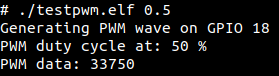
\includegraphics[width=6.25cm]{13tests/pwm/pwm_50}}}%
	\qquad
	\subfloat[\centering Generated PWM signal. ]{{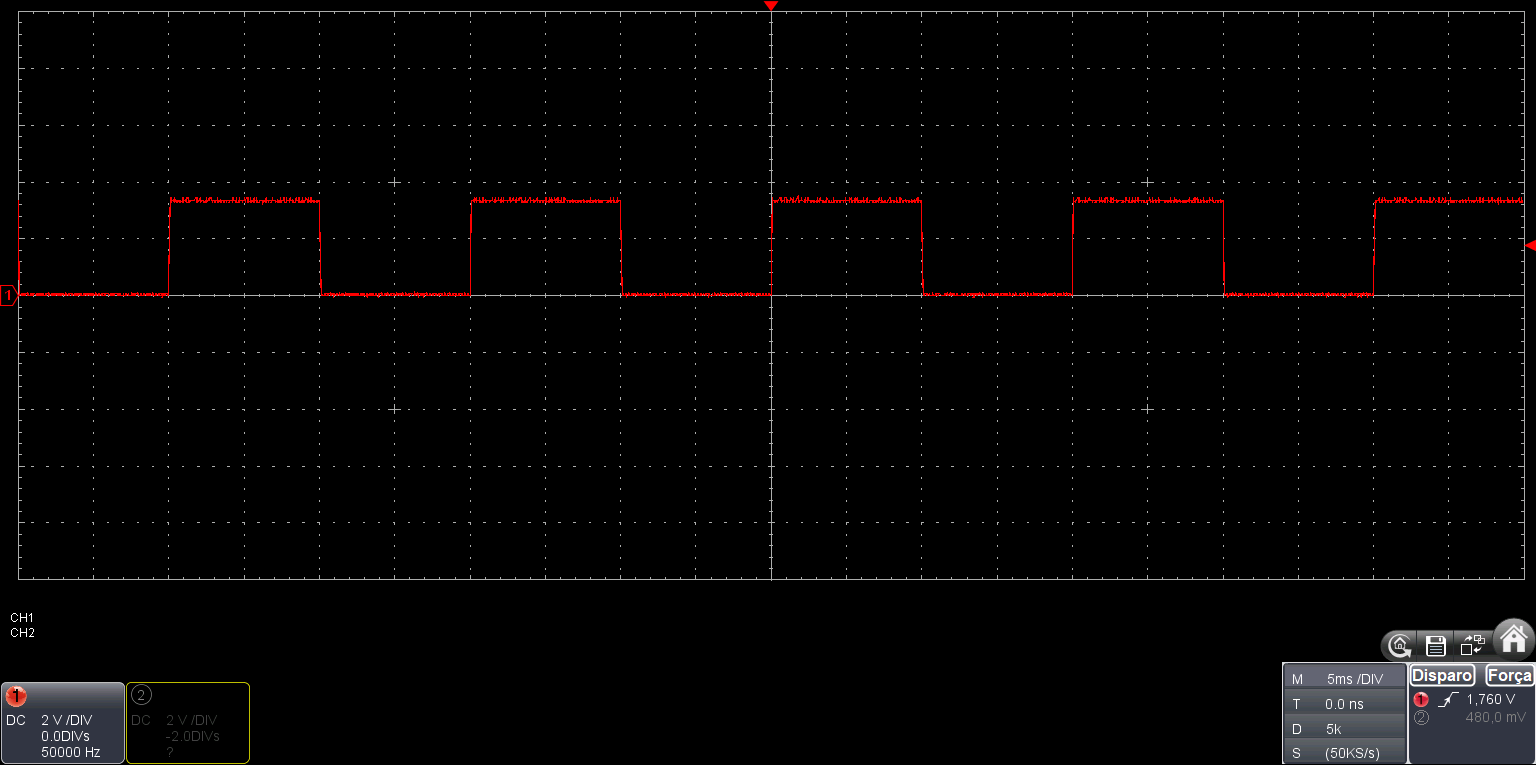
\includegraphics[width=12cm]{13tests/pwm/Duty_50}}}%
	\caption{Test PWM control: PWM at 50\% duty cycle.}%
	\label{fig:pwm_50}%
\end{figure}

In figure \ref{fig:pwm_25} is shown the a PWM generated signal with \verb+25 %+ duty cycle, with output on the GPIO 18. In figure \ref{fig:pwm_25} (a) one can check that the field \verb|PWM data| is equal to \verb+RANGE*0,25+.

\begin{figure}[H]%
	\centering
	\subfloat[\centering Set duty cycle to 25\%. ]{{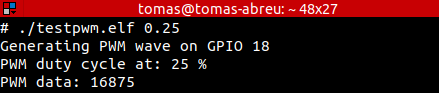
\includegraphics[width=6.25cm]{13tests/pwm/pwm_25}}}%
	\qquad
	\subfloat[\centering Generated PWM signal. ]{{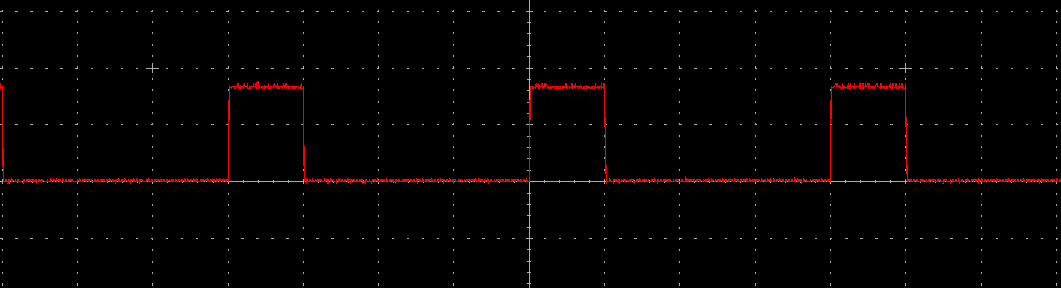
\includegraphics[width=12cm]{13tests/pwm/Duty_25}}}%
	\caption{Test PWM control: PWM at 25\% duty cycle.}%
	\label{fig:pwm_25}%
\end{figure}

%**********************************************************
\section{Motion Detector}

As mentioned before, for the motion detector, the PIR HC-SR501, it was implemented a device driver. After insert its module in the kernel using the \verb|insmod| command, one can test if the sensor detects movement, using a small test code. In figure \ref{fig:testpir}, one can see the execution of the program that shows that the sensor detected movement.

\begin{figure}[H]
	\centering	
	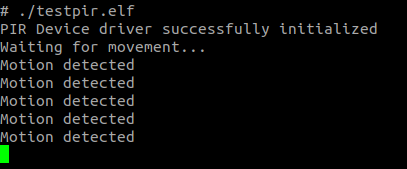
\includegraphics[width=.5\textwidth]{13tests/pir/testpir}
	\caption{Test PIR HC-SR501 module: Detection of movement.}
	\label{fig:testpir}
\end{figure}

In figure \ref{fig:pirMount}, it is shown the the movement sensor connected to the Raspberry Pi. During the tests, it was noticed that the sensor must be stable to not detect false positives. Furthermore, there is a insignificant delay in the detection of the movement, despite the attempts to adjust, using the potentiometers in the module.

\begin{figure}[H]
	\centering	
	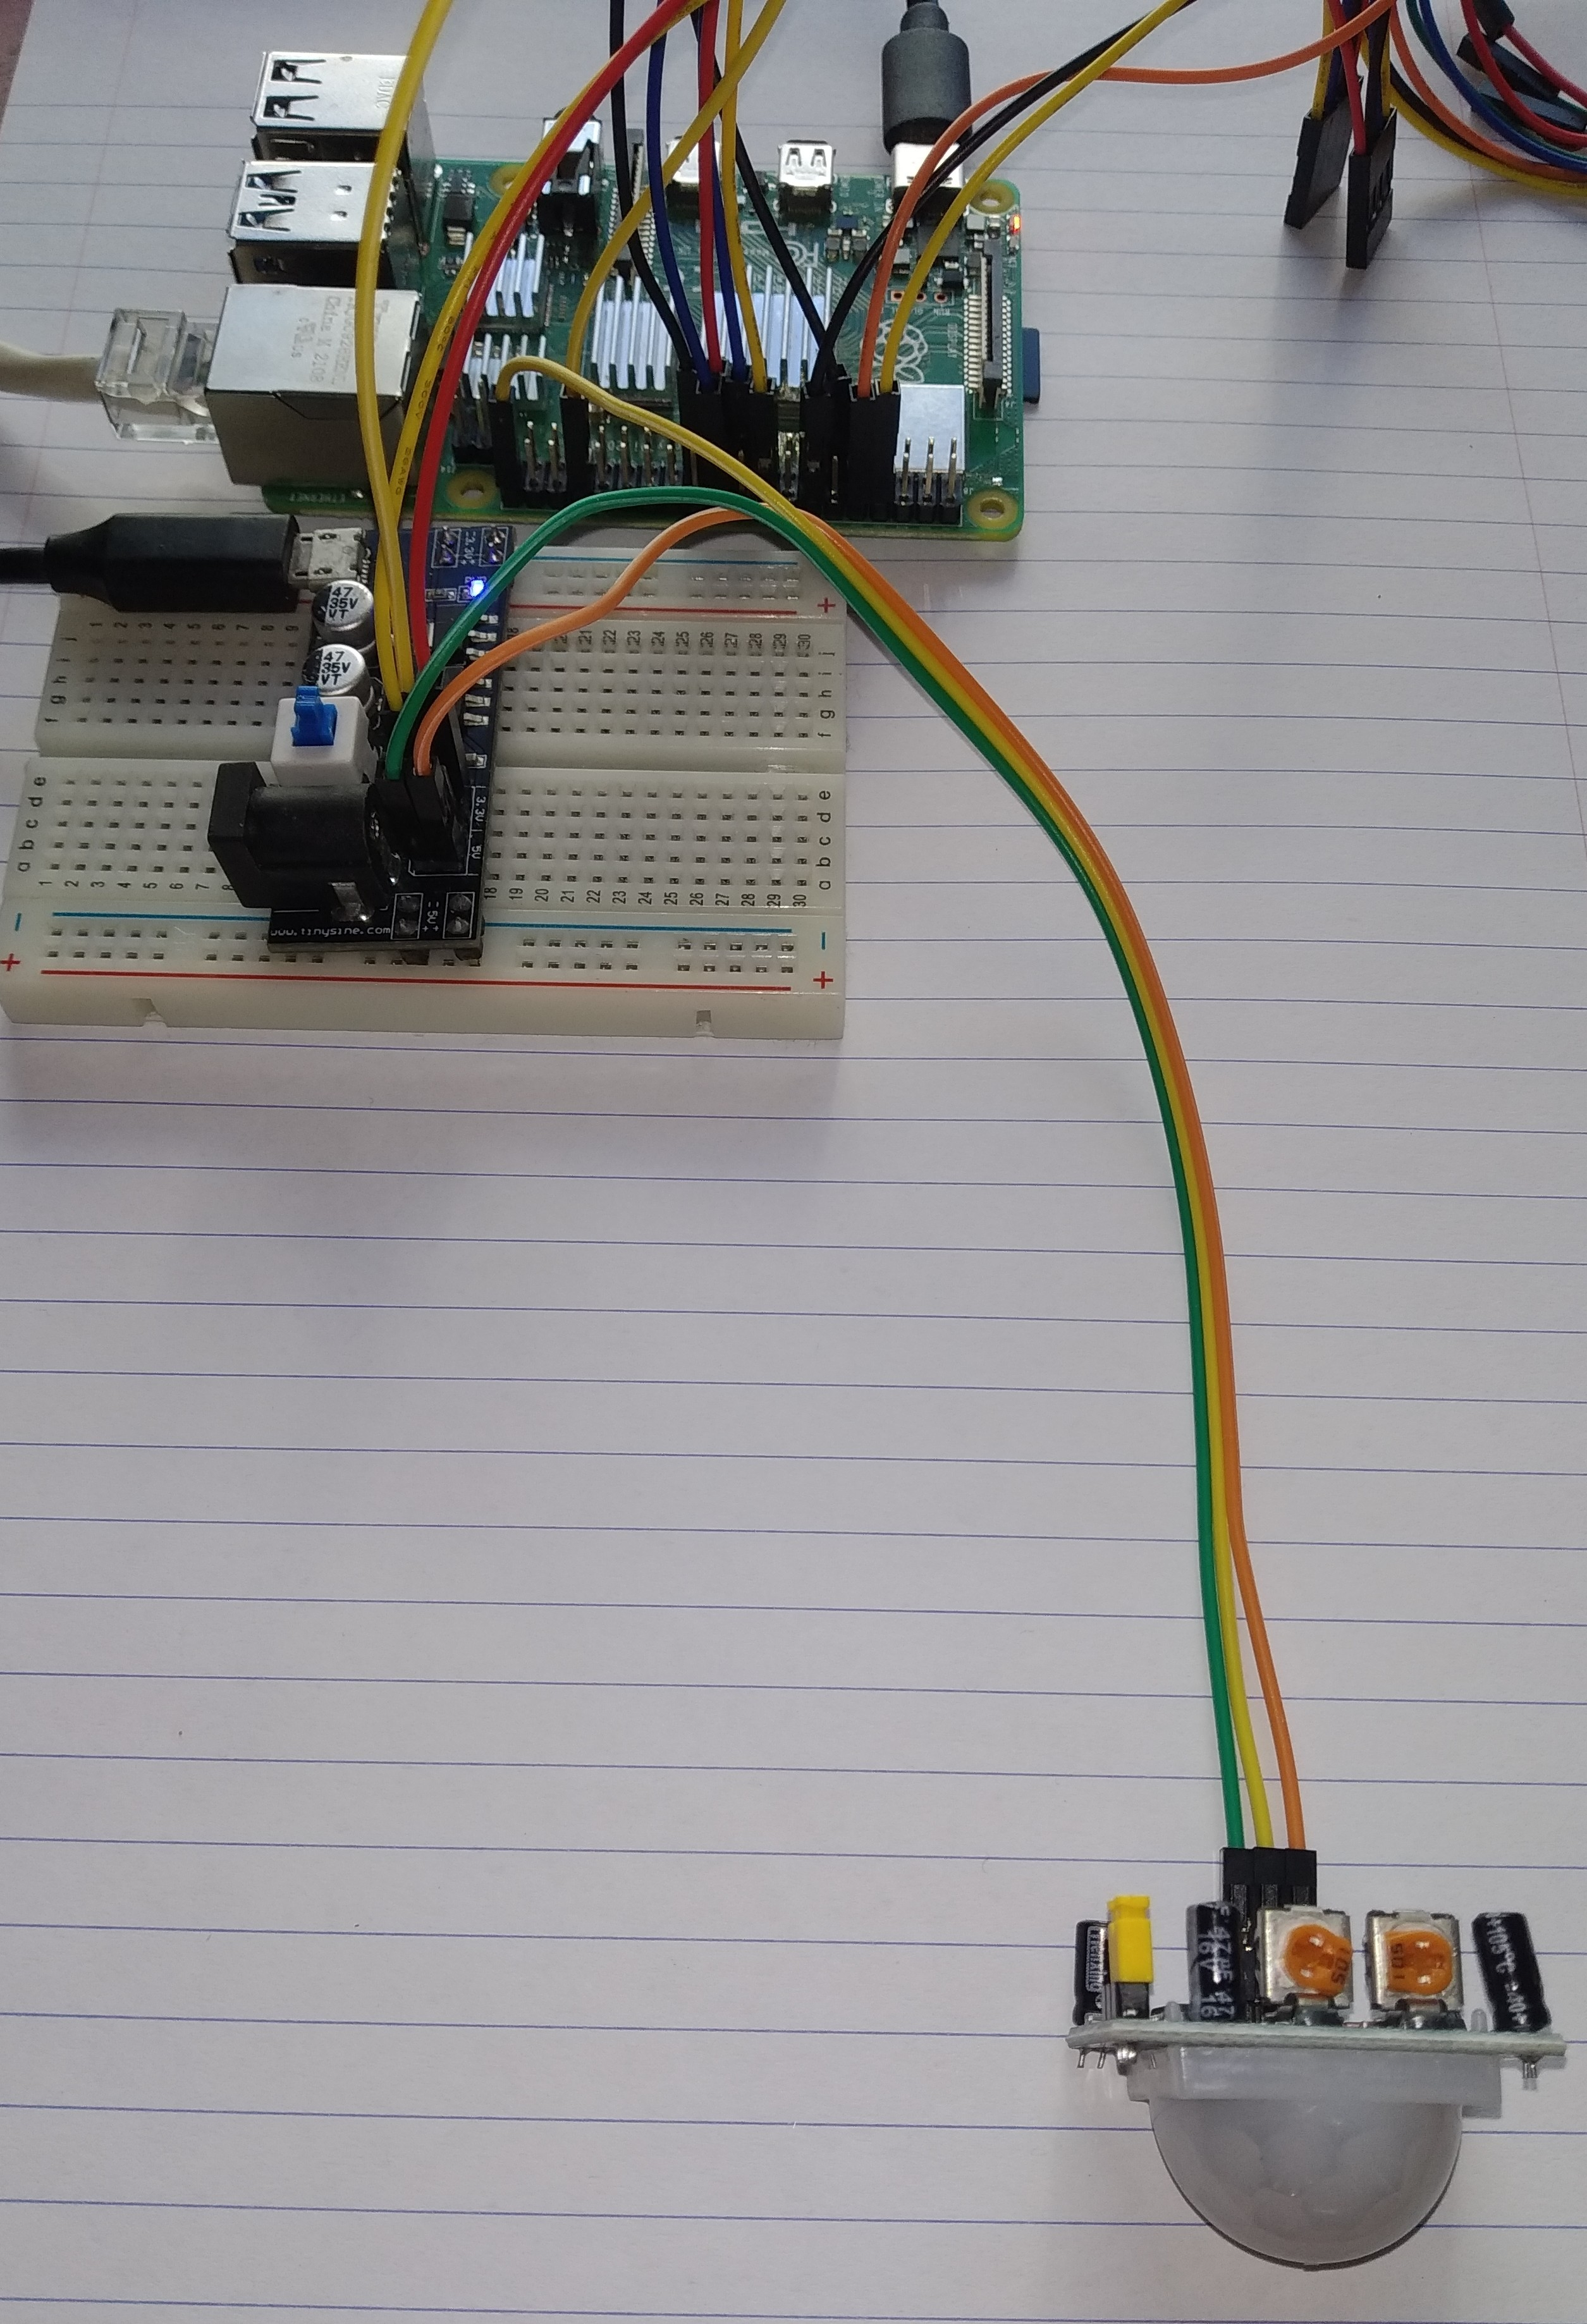
\includegraphics[width=.4\textwidth]{13tests/pir/pir}
	\caption{Test PIR HC-SR501 module: Montage.}
	\label{fig:pirMount}
\end{figure}